\documentclass[10pt,a4paper]{article}

\usepackage{amsmath}        % mathematics
\usepackage{hyperref}       % hyper-links
\usepackage{lipsum}         % random text
\usepackage{listings}       % boxed file lists
\usepackage{tikz}           % graphics
\usepackage{booktabs}       % for table rendering
\usepackage{pgfplotstable}  % plot a table from .csv files
\usepackage{pgfcalendar}    % for date columns

\title{\LaTeXe{} Article Example}
\author{Frank Jung}
\date{\today}

\lstset{
  basicstyle=\small,
  frame=single,
  tabsize=2,
  showspaces=false,
  showtabs=false,
  numbers=left,
  numberstyle=\tiny,
  numberblanklines=false
}

\begin{document}

\pagenumbering{gobble}
\maketitle
\newpage

\pagenumbering{roman}
\tableofcontents{}
\listoffigures
\listoftables
\newpage

\pagenumbering{arabic}
\newpage

\newcommand{\sectionbreak}{\clearpage}

\section*{Introduction}
\addcontentsline{toc}{section}{Introduction}

This is a \LaTeXe{} document to provide some examples of usage. To fill out the
document there are \href{http://www.lipsum.com/}{Lorem Ipsum} paragraphs.

\lipsum[1]

\sectionbreak{}

\section*{Equations}
\addcontentsline{toc}{section}{Equations}

Equations can be included into the document in a number of ways. The first
example can be a either number or unnumbered equation.

\paragraph{}
The mass-energy equivalence is described by the famous equation:

\begin{equation}
  E = mc^2
\end{equation}

\paragraph{}
Equations can also be inline. For example, $f(x) = x^2$. An more text here.
\lipsum[2]

\sectionbreak{}

\section*{Gnuplot}
\addcontentsline{toc}{section}{Gnuplot}

Plots can be included or rendered inline. The following example uses
\href{http://www.gnuplot.info/}{Gnuplot} to graph functions.

\subsection*{Inline Gnuplot}
\addcontentsline{toc}{subsection}{Inline Gnuplot}

To render this inline plot ensure that:
\begin{itemize}
  \item \texttt{gnuplot} is installed
  \item \texttt{latexmf} requires the \texttt{-shell-escape} option
\end{itemize}
This renders as:

\begin{figure}[h]
  \centering
  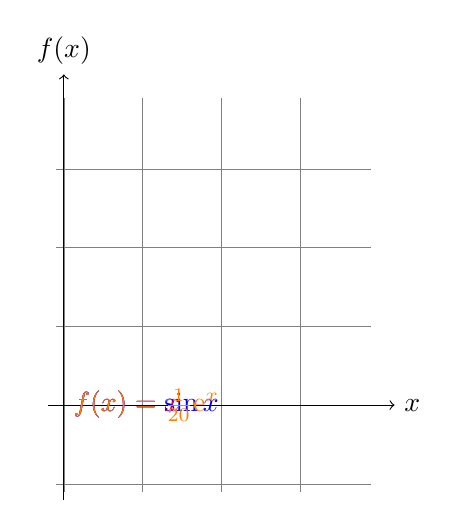
\begin{tikzpicture}[domain=0:4]
    \draw[very thin,color=gray] (-0.1,-1.1) grid (3.9,3.9);
    \draw[->] (-0.2,0) -- (4.2,0) node[right] {$x$};
    \draw[->] (0,-1.2) -- (0,4.2) node[above] {$f(x)$};
    \draw[color=red] plot[id=x] function{x}
      node[right] {$f(x) =x$};
    \draw[color=blue] plot[id=sin] function{sin(x)}
      node[right] {$f(x) = \sin x$};
    \draw[color=orange] plot[id=exp] function{0.05*exp(x)}
      node[right] {$f(x) = \frac{1}{20} \mathrm e^x$};
  \end{tikzpicture}
  \caption{Inline Gnuplot example}
\end{figure}
The code to generate this plot is:
\begin{figure}[h]
  \begin{lstlisting}[language=TeX]
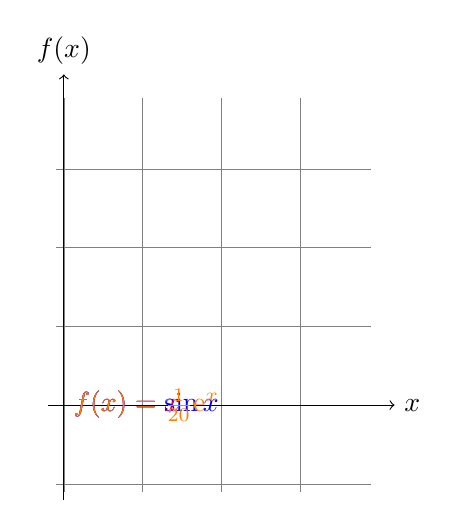
\begin{tikzpicture}[domain=0:4]
  \draw[very thin,color=gray] (-0.1,-1.1) grid (3.9,3.9);
  \draw[->] (-0.2,0) -- (4.2,0) node[right] {$x$};
  \draw[->] (0,-1.2) -- (0,4.2) node[above] {$f(x)$};
  \draw[color=red] plot[id=x] function{x}
    node[right] {$f(x) =x$};
  \draw[color=blue] plot[id=sin] function{sin(x)}
    node[right] {$f(x) = \sin x$};
  \draw[color=orange] plot[id=exp] function{0.05*exp(x)}
    node[right] {$f(x) = \frac{1}{20} \mathrm e^x$};
\end{tikzpicture}
  \end{lstlisting}
  \caption{LaTeX snippet for embedded Gnuplot}
\end{figure}

\pagebreak[4]

\subsection*{External Gnuplot}
\addcontentsline{toc}{subsection}{External Gnuplot}

This example includes an externally rendered Gnuplot.

\begin{figure}[h]
  \centering
  \includegraphics{plot}
  \caption{External Gnuplot example}
\end{figure}

The code to generate this plot is:
\begin{figure}[h]
  \begin{lstinputlisting}[language=Gnuplot]{plot.gnuplot}
  \end{lstinputlisting}
  \caption{Gnuplot source code}
\end{figure}

\sectionbreak{}

\section*{Tables}
\addcontentsline{toc}{section}{Tables}

The following example shows how to reproduce table data from an external CSV source.

\begin{table}[h]
\label{table1}
  \begin{center}
    \pgfplotstabletypeset[
      col sep=comma,
      every head row/.style={before row=\toprule,after row=\midrule},
      columns/file/.style={column name=\textit{File Name},column type=l,string type},
      columns/size/.style={column name=\textit{Size (Bytes)},column type=r,int type},
      columns/changed/.style={column name=\textit{Date Changed},column type=r,date type={\day\ \monthshortname\ \year}},
      every last row/.style={after row=\bottomrule},
    ]{table.csv}
    \caption{Generate table from CSV file}
  \end{center}
\end{table}

\lipsum[3]

\sectionbreak{}

\section*{Makefile}
\addcontentsline{toc}{section}{Makefile}

This project use a \href{https://www.gnu.org/software/make/}{Makefile} to build
a PDF from this document. The Makefile is very simple:

\begin{figure}[h]
  \lstinputlisting[language=make,tabsize=4]{Makefile}
  \caption{Makefile source code}
\end{figure}

\sectionbreak{}

\section*{Git}
\addcontentsline{toc}{section}{Git}

\paragraph{}
Include another TeX document into this one. The following sections are
contained in the document, \texttt{attachment.tex}.

\subsection*{Restore older version of a file}
\addcontentsline{toc}{subsection}{Restore older version of a file}

Given a list of commits on a file, revert to an older state of the
file and commit as a new change.

\subsubsection*{Method}
\addcontentsline{toc}{subsubsection}{Method}

\begin{itemize}
\item list commit history of file to get commit hashes
\item checkout older commit for that file
\item  check local file has changed, so can commit as new change
\end{itemize}

\subsubsection*{Detail}
\addcontentsline{toc}{subsubsection}{Detail}

This is the current version of our test file:
\begin{minted}{bash}
test
changed
exit-code
\end{minted}
To determine where to restore to, list the commit history of file to get commit
hashes:
\begin{minted}{bash}
git log --oneline README.md
dc9de3e latest change
dbc5cca another change
fe66fc4 new change
c56ac1c initial
\end{minted}
Lets restore to a version 2 commits back. To checkout older commit
for that file:
\begin{minted}{bash}
git checkout dbc5cca README.md
\end{minted}
Check that the local file has changed, so can commit as new change:
\begin{minted}{bash}
test
changed
exit-code
another change
\end{minted}
You can now add changed file and commit this version as a new commit:
\begin{minted}{bash}
git status
On branch master
Changes to be committed:
  (use "git reset HEAD <file>..." to unstage)

	modified:   README.md
\end{minted}


\paragraph{}
After included attachment.

\end{document}
